\documentclass[a4paper,twocolumn,12pt]{article}
\usepackage[letterpaper,scale=0.875,right=1.3cm,top=2cm]{geometry} % 
\usepackage[utf8]{inputenc}
\usepackage{pxfonts}
\usepackage{wasysym} % symbols
\usepackage{abstract}
\usepackage{parskip}
\usepackage{microtype}
\usepackage{verbatim}   
\usepackage[hyperindex=false,breaklinks=false,colorlinks=false,linkcolor=false]{hyperref}
\usepackage{graphicx}
%\def\sym##1{\ifmmode^{##1}\else\(^{##1}\)\fi}
\usepackage{titlesec}
\usepackage{xcolor}
%no quitar nada
\hypersetup{
    colorlinks=true,
    linkcolor=carnelian, % Color para enlaces internos
    urlcolor=carnelian,   % Color para enlaces URL
    citecolor=carnelian, % Color para citas bibliográficas
}
\usepackage{float}
\usepackage{graphicx}
\usepackage{blindtext}% only for dummy text
\usepackage{fancyhdr}
\usepackage{titling}
\usepackage{caption}
\usepackage{dcolumn}

\captionsetup[table]{
  position=above,
  justification=raggedright,
  labelsep=newline, % <<< label and text on different lines
  singlelinecheck=false % <<< raggadright also when the caption is shorter
                        % than a single line
}
\usepackage[document]{ragged2e}
\usepackage[affil-sl]{authblk} 
\usepackage{mathptmx}  %Times new Roman


%$$$$$$$$$$$$$$$$$$$$$$$$$$$$$$$$$$$$$$$$$$$$
\usepackage{orcidlink}







\setlength{\columnsep}{1cm}
\renewcommand{\refname}{REFERENCES}
\renewcommand{\figurename}{Fig.}


% Keywords command
\providecommand{\keywordsSpan}[1]
{
  \small	
  \textbf{\textit{Palabras Clave:}} #1
}

\providecommand{\keywordsEng}[1]
{
  \small	
  \textbf{\textit{Keywords:}} #1
}





\pagestyle{fancyplain}% <- pagestyle fancyplain
\fancyfoot[C]{}
\renewcommand\plainheadrulewidth{.4pt}% headrule on plain pages
%\fancyhf{}
\fancyhead[C]{Fraud Detection}
\rhead{}
\lhead{}
\rfoot{}



\definecolor{carnelian}{rgb}{0.7, 0.1, 0}

%%%%%%%% FORMATO DE LAS SECCIONES Y SUBSECCIONES %%%%%
\titleformat*{\section}{\fontsize{14}{1}\bfseries\color{carnelian}}


\titleformat*{\subsection}{\fontsize{13}{1}\bfseries\color{carnelian}\itshape}


\titlespacing*{\section}
{0pt}{1cm}{0.2cm}

\titlespacing*{\subsection}
{0pt}{1cm}{0.2cm}




 
\makeatletter
\long\def\@makecaption#1#2{
\vskip\abovecaptionskip
\sbox\@tempboxa{#1. #2}
\ifdim \wd\@tempboxa >\hsize
#1. #2\par
\else
\global \@minipagefalse
\hb@xt@\hsize{\hfil\box\@tempboxa\hfil}
\fi
\vskip\belowcaptionskip}
\makeatother


\fancypagestyle{plain}
{%
\fancyhf{}
\renewcommand{\headrulewidth}{0.5pt}
\renewcommand{\footrulewidth}{0pt}
\fancyheadoffset[LO]{-0.42\textwidth}
\fancyhead[RO]{{
\includegraphics[scale=0.025]{Figuras/aualogo} }} 
\fancyhead[LO]{American University Of Armenia\\ \emph{Bachelors Degree In Data Science}}
\fancyfoot[CO]{\footnotesize{\thepage}}
}
\fancyfoot[CO]{\footnotesize{\thepage}}


\usepackage{balance}
\usepackage{flushend}
\newcommand{\balancecolumns}{%
  \vfill\eject
  \global\@colht = \textheight
  \global\ht\@cclv = \textheight}
    

%%%%%%%%%%%%%%%%%%%%%%%%%%%%%%%%%%

\date{}  

{\title{
\vspace*{1cm}
\Large{ Capstone Paper \\
\large{\textcolor{carnelian}{\emph{Fraud Detection Tool}}}
\\[0.2cm]}}}

\usepackage{amsmath}
\usepackage{graphicx}
\begin{document}

\onecolumn % Start with one column for the title page
\thispagestyle{empty} % Remove page numbers
% Logo at the top right
\begin{tikzpicture}[remember picture,overlay]
 \node[anchor=north east,inner sep=2pt] at (current page.north east) {
    
\includegraphics[width=4cm]{Figuras/aualogo.png}
  };
\end{tikzpicture}

\vspace*{6cm} 



\begin{center}
    {\Large\textbf{Capstone Paper}}\\[0.5cm] % Title
    {\Large\textbf{Fraud Detection Tool}}\\[1.5cm] % Subtitle
    
    {\large Aleksandr Shaghbatyan, Gurgen Hovakimyan}\\[1cm] % Authors
    
    {\large BS in Data Science}\\[1cm] % Degree
    
    {\large American University of Armenia}\\[1cm] % University
    
    {\large May 9, 2024} % Date
\end{center}

\newpage

\vspace*{3cm} 

% Table of Contents
\tableofcontents

\newpage
\twocolumn % Return to two columns for the rest of the document



% \begin{document}

\twocolumn
[
\begin{@twocolumnfalse}
% \maketitle
% \begin{flushleft}
%     \textbf{Update Date:} \today\\
% \end{flushleft}


\vspace*{0.3cm}





\renewcommand{\abstractname}{\textcolor{carnelian}{Abstract}}
\begin{abstract}
\vspace*{0.5cm}
\fontsize{13pt}{12pt}\selectfont
\justify

Utilizing machine learning algorithms has proven to be a potent method for managing risk and preventing financial fraud. However, the requirement for coding expertise and deep knowledge of machine learning stands as a barrier for users who need such skills. This study offers an innovative, user-friendly framework that uses machine learning to address this difficulty. The paper studies the performance of three machine learning models, Random Forest, SVM, and XGboost, to classify, detect, and predict fraudulent transactions. 

\keywordsEng{Fraud detection, machine learning, risk management tool, data cleaning, data visualization, classification, machine learning algorithms, streamlit, random forest, XGboost, SVM, finance, detection models, dynamic environments.}

\end{abstract}
\vspace*{0.5cm}
\headrule
\vspace*{0.5cm}


\end{@twocolumnfalse}]

\section{Introduction}

\subsection{Risk Management Problem}

\justifying

Risk management is getting progressively more comprehensive in today's constantly developing online information technologies. Credit card payments in 2018 totaled \$44.7 billion in the U.S. alone, according to The 2019 Federal Reserve Payments Study. The speed at which these transactions process is awe-inspiring. Credit cards can settle 5,000 transactions per second.\cite{cardrates} Moreover, Credit card usage has increased from 18\% to 23\%, from 2016 to 2018.\cite{cardrates} The rapid growth of online banking follows an increasing number of frauds. According to the 2017 Financial Institutions Payments Fraud Mitigation Survey by the Federal Reserve Bank of Minneapolis, Ninety-six percent of the respondents are debit card issuers, and 77\% of credit card issuers experienced card fraud losses in 2016. Loss increases are more prevalent on debit and credit cards than on other payment types. Fraud losses increased in 2016 compared to 2015 on debit cards (63\% of FIs) and credit cards (41\% of FIs).\cite{dorphy20182017}


Governmental institutions suffer from fraudulent transactions as well. The Institute of International Finance and Deloitte LLP White Paper report, Though this global fight against financial crime is critical, the current financial crime risk management framework is not as effective as it should or could be. For example, each year, the amount of money laundered globally  is estimated to be 2\% to 5\% of global GDP, or between 715 billion EUR and 1.87 trillion EUR.\cite{shepard2019global}  The UN estimated US\$800 billion to US\$2 trillion is laundered every year. But unfortunately, about 90\% of this amount remains undetectable today.\cite{chairunnisa2023tracking}


In this new landscape, traditional fraud detection approaches such as rule-based engines have largely become ineffective. AI and machine learning solutions using graph computing principles have gained significant interest.\cite{kurshan2020financial} Execution of an accurate and effective fraud detecting system is of major importance to all financial card issuing bodies. Several ways are based on approximate reasoning, AI, Data mining, sequence alignment that identifies regions of similarities, inheritable programming, etc., which are highly used in detecting these credit card frauds.\cite{9913607}


The project aims to study and provide non-technical users with data processing, data visualization, and various autonomation methods for identifying and predicting fraudulent transactions. It is done using Streamlit to create a user-friendly interface and a shareable app. The application has three tabs: Data Cleaning, Data Visualization, and Risk Identification.



 
\subsection{Research Questions}

This paper aims to create a user-friendly environment for risk managers and other specialists in the fraud detection field, allowing them to improve their work quality and decrease the time for data preprocessing. For this purpose, the following research questions have been defined.

\textbf{Research Question 1}: Will the user-friendly framework let non-technical users analyze their data effectively?

\textbf{Research Question 2}: How do the implemented models behave in terms of fraud detection problems?

To address the above-mentioned research questions, we applied the following methods.

\textbf{Addressing Research Question 1:} The project was implemented using Streamlit to find the answer to the first research question. Users can clean, process, visualize, and use classification machine learning algorithms to analyze their specific data by simply choosing the corresponding tab. The application does not require any coding skills. The results are discussed in the following sections. 

\textbf{Addressing Research Question 2:} To address the second research question, three machine learning algorithms — random forest, XGboost, and SVM—were implemented and tested on a specific real dataset. The results are discussed in the next sections. 


\subsection{Structure Of The Paper}

The remainder of this paper is structured as follows:

\textbf{Section 2, Literature Review} This section provides a thorough literature review, delving into papers that address similar and the same problems. It includes detailed information about dealing with outlier removals, models used to solve fraud detection tools, and their results, ensuring the validity of our research. 


\textbf{Section 3, Data Collection} This section provides a detailed account of the datasets used, including their characteristics, sources, and additional information. It ensures a clear understanding of the data used in our research. 

\textbf{Section 4, Related Work} This section covers the information needed to understand the evaluation of the models that were used to accomplish the fraud detection problem. Different metrics of model evaluation are described and explained. 

\textbf{Section 5, Tabs} This section describes the data cleaning, data visualization, and model development tabs that exist in the application. It covers the functionality information and methods that the application uses to operate.

\textbf{Section 6, Conclusion And Future Work} This section describes the conclusion made based on the results and contains information about the future work that can be done to develop the application and improve the results. 


\section{Literature Review}

\subsection{Literature Review For Outlier Detection}

Outlier detection has a wide range of applications, including data quality monitoring, identifying price arbitrage in finance, detecting cybersecurity attacks, healthcare fraud detection, banknote counterfeit detection, and more.\cite{outlier-detection} There are several ways to deal with outliers. Box plot plots the \(Q_1\) (25th percentile), \(Q_2\) (50th percentile or median) and \(Q_3\) (75th percentile) of the data along with \(Q_1-1.5 \times (Q_3-Q_1\) and \(Q_3+1.5 \times (Q_3-Q_1)\). Outliers, if any, are plotted as points above and below the plot.\cite{boxplot-outlier} IQR method: The data points that fall below \(Q_1-1.5 \times IQR\) or above the third quartile \(Q_3 + 1.5 \times IQR\) are outliers, where \(Q_1\) and \(Q_3\) are the 25th and 75th percentile of the dataset, respectively. IQR represents the inter-quartile range and is given by \(Q_3 - Q_1\).\cite{the-data-points}

\subsection{Logistic Regression}

 Logistic regression is a technique used to predict a binary outcome variable. This technique does not demand that explanatory variables follow a normal distribution or are correlated. Using the logistic function, it models the dependent variable and predicts the probability of a target variable.\cite{chang2007intrusion}

The nature of these variables is dichotomous. It is represented as an equation that combines the input values linearly using the coefficient values to predict an output. The sigmoid function is used in equation\cite{9913607}  \(S(X) = \frac{1}{1+e^x}\)

Logistic regression is preferred in these scenarios to build the classifier due to its better efficiency in detecting frauds based on the data isolation provided to binary classes.\cite{9913607}
Advantages of Logistic regression :
Logistic regression is easy to implement but more advanced than linear regression because linear regression is not good with widely distributed data. 
No assumptions were made regarding the distribution of classes in the feature space.
It is easier to extend to multiple classes in logistic regression.
It works well with the classification of unknown data.\cite{9913607}
Logistic regression was used to create numeric fraud detection tools. Implementing logistic regression resulted in a 92\% accuracy score. F1-Score, Recall, and Precision were 0.08, 0.76, and 0.04, respectively.

\subsection{Decision Tree}

Decision tree is a nonlinear classification technique that divides a sample into increasingly smaller subgroups using a collection of explanatory variables. At each branch of the tree, the process iteratively chooses the explanatory variable that, by a predetermined criterion, has the strongest correlation with the outcome variable.\cite{afriyie2023supervised} The advantage of the suggested method is that it is easy to implement, understand, and display. However, a disadvantage of this system is the requirement to check each transaction individually. Nevertheless, similarity trees have given proven results.\cite{fan2004using} The decision tree algorithm has the benefit of not needing feature scaling, being robust to outliers, and handling missing values automatically. It is quicker to train and is very good at resolving classification and prediction problems. The decision tree uses the Gini index, information gain, and entropy as a metric for classification into two or more nodes.\cite{afriyie2023supervised} The experiment of implementing a decision tree algorithm for predicting fraud credit card transactions resulted in a 92\% accuracy score with 0.09 F1-Score, 0.93 Recall, and Precision of 0.05 estimates.

\subsection{Unsupervised Learning Methods}

Other than supervised learning approaches like the abovementioned Logistic regression and decision tree algorithms, there are also unsupervised learning methods. Such methods do not require labeled data. This presents a significant advantage, as fraudulent transactions are often rare, and labeling them can be expensive and time-consuming.\cite{carcillo2021combining}  Moreover, unsupervised learning has one more advantage, which is its adaptability. Unsupervised techniques can adjust to new fraud tactics without constant retraining.\cite{kazeemfraud}
However, these techniques also face limitations. The main challenge is the high rate of false positives. In other words, these models may identify legitimate transactions as fraudulent or identify clusters containing both valid and fraudulent activities. Additionally, unsupervised techniques might need help to provide the granular detail required to identify specific fraudulent transactions or the individuals involved.\cite{kazeemfraud}




\section{Data Collection}

\subsection{First Dataset}

As the paper aims to solve multiple challenges, two different datasets were used for the following paper. Both of them were taken from the Kaggle open-source web page. The first dataset is called Credit Card Fraud Detection. The dataset contains information about transactions made by credit cards in September 2013 for two days by European cardholders. It includes 284,807 transactions, out of which 492 were labeled as fraudulent. Due to confidentiality, the original features except 'Time' and 'Amount' were changed to ( V1, V2, ... V28 ). The 'Class' feature only takes values of 0 and 1, which labels legitimate or fraudulent transactions accordingly.
\begin{figure}[h]
\centering
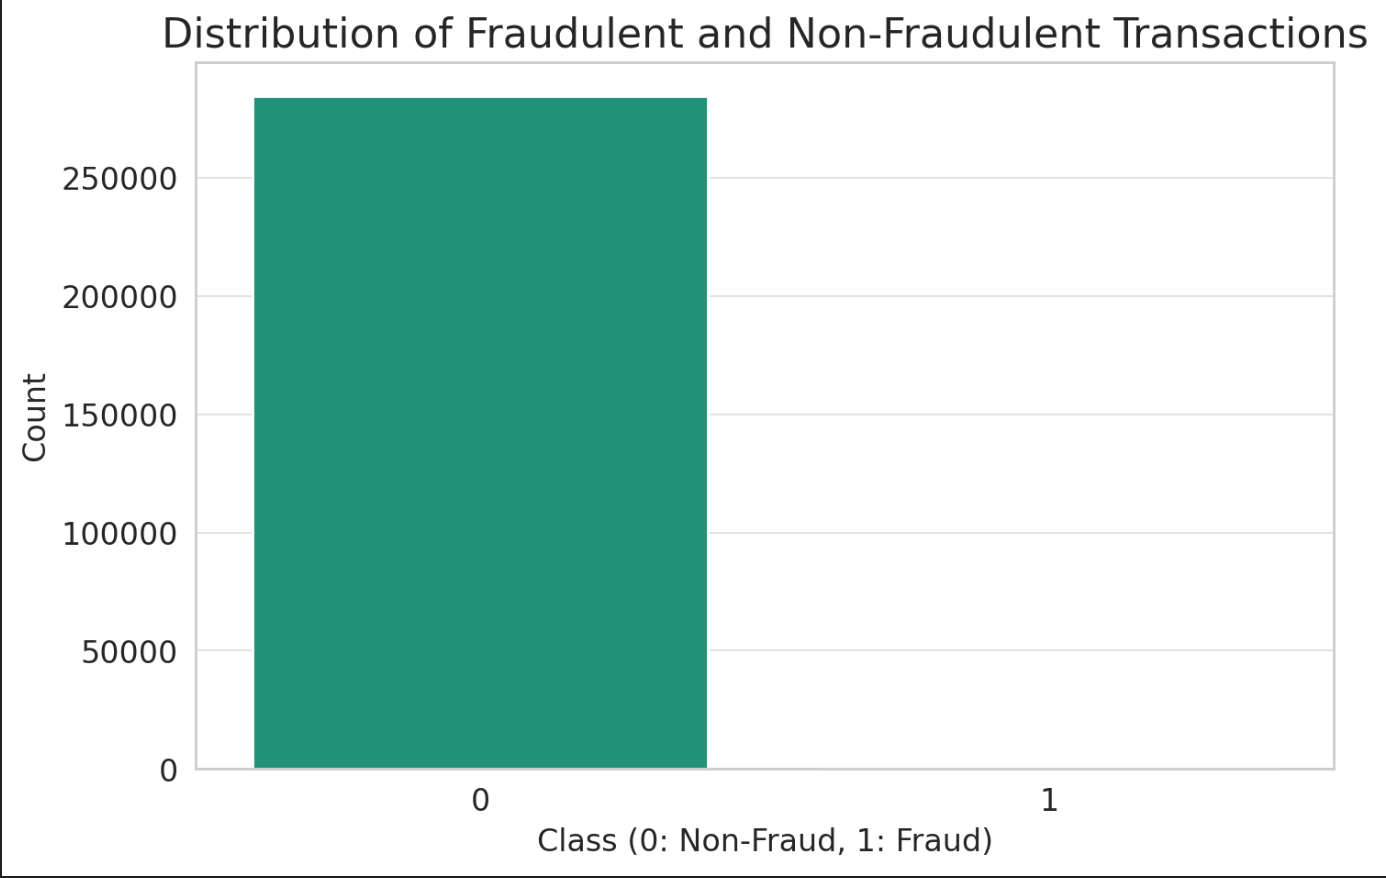
\includegraphics[width = 0.4\textwidth]{Figuras/Histogram of fraud.png} 
\caption{Histogram of the fraud and non-fraud transactions in the dataset}
\end{figure}

Fig. 1. shows a significant imbalance between classes non-fraudulent and fraudulent transactions

\begin{figure}[h]
\centering
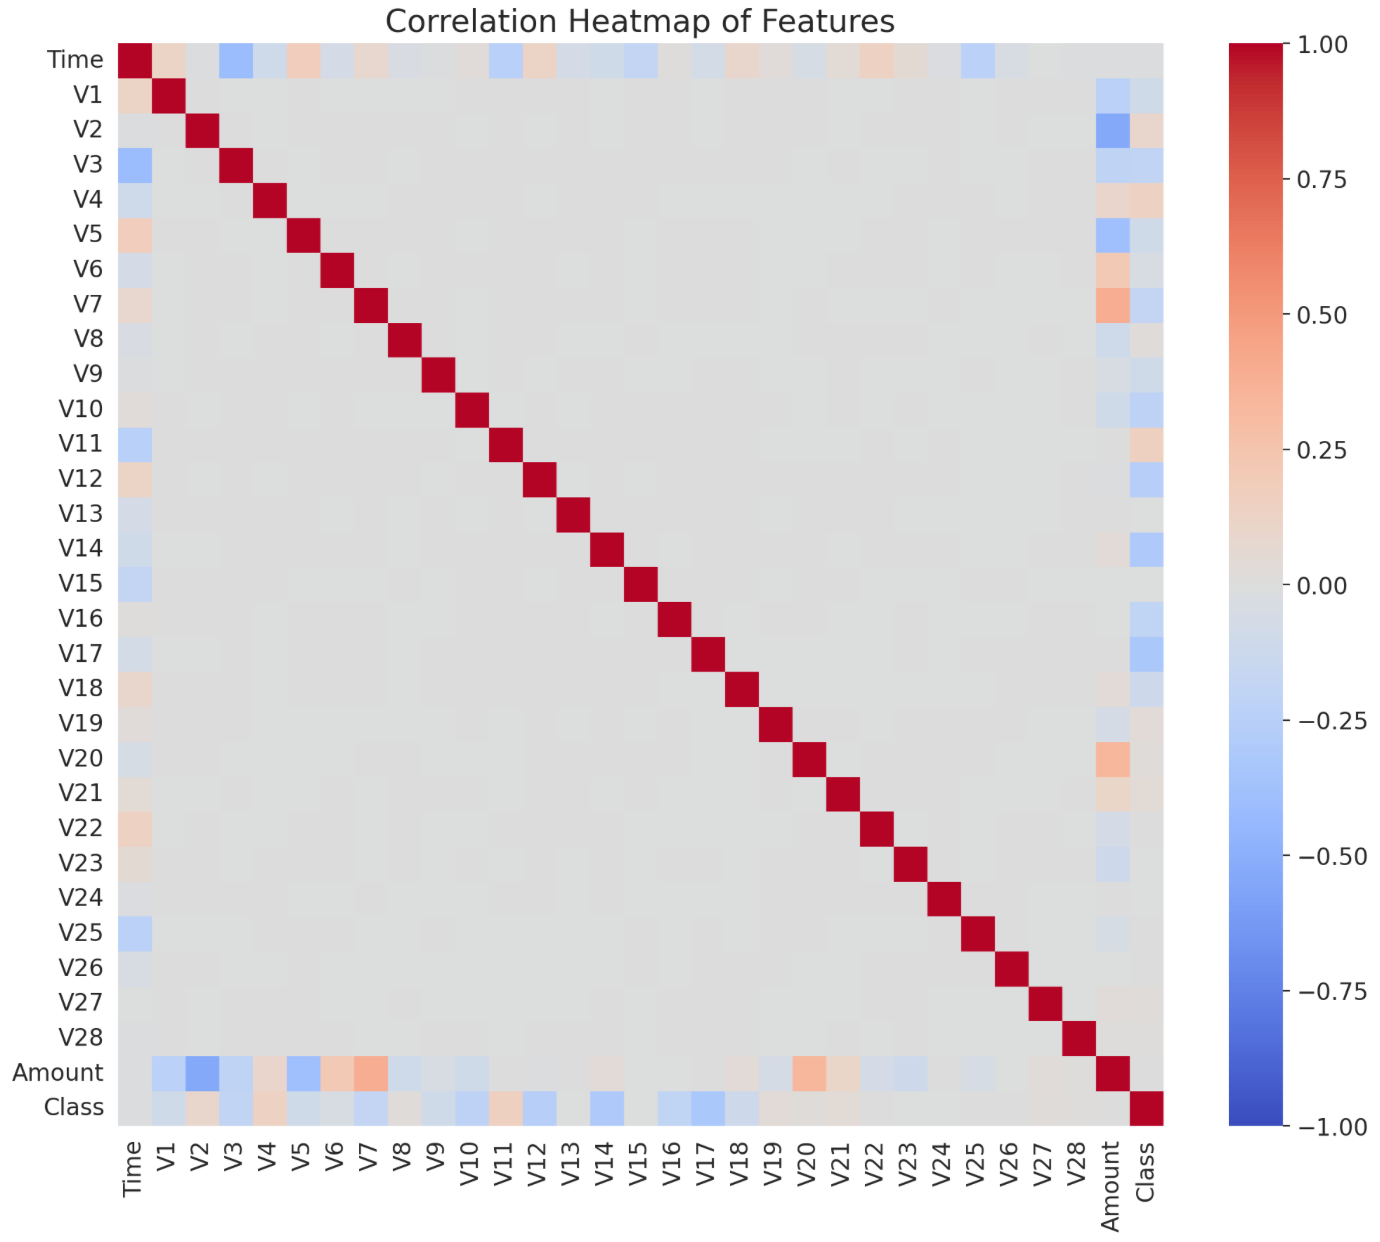
\includegraphics[width = 0.4\textwidth]{Figuras/HeatMap of Fdata.png}
\caption{Heatmap of all features in the dataset}
\end{figure}

Fig. 2. shows that the features do not show strong correlation with the feature class, which indicates that detection of fraudulent transactions requires combining multiple features  

\subsection{Second Dataset}



As the first dataset was cleaned before publishing, the second dataset has been chosen for the data cleaning part. The dataset is called the Vehicle Dataset. It contains information about used cars for sale. The dataset's features are name, year, selling\_price, km\_driven, fuel, seller\_type, transmission, owner, mileage, engine, max\_power, torque, and seats.



\section{Related Work}


    
The model evaluation is described by the accuracy score, confusion matrix, and classification matrix, which includes precision, recall, f1-score, and support. 

\begin{itemize}

    \item Accuracy is the ratio of actual results to all occurrences. It shows the probability that the model would correctly anticipate a specific outcome out of all the predictions it has made. 
    \item The confusion matrix is a visualization tool that displays the number of true positive, false positive, true negative, and true positive values the model predicted.
    \item The precision score shows the percentage of correctly predicted values. It is calculated by dividing true positive values into the sum of false positive and true positive values. 
    \item Recall shows the percentage of the model's ability to catch positive values correctly. The recall score is calculated by dividing the true positive values by the sum of true positive and false negative values. 
    \item F1-score shows the weighted harmonic mean of precision and recall. The formula of the f1 score is \(2 \times \frac{\text{Recall} \times \text{Precision}}{\text{Recall}+ \text{Precision}}\) The best score for f1 is 1, and the worst one is 0
    \item Support shows the number of actual class instances in the given dataset. This metric diagnoses the model's evaluation process and does not change when the model is switched.\cite{related_work}

\end{itemize}

\section{Tabs}
\subsection{First Tab}

The first tab of the project provides users with the opportunity to process the data. After uploading a dataset, it finds the missing values in each column and returns the number. After getting this information, the user can fill in these missing values using methods like mean, median, mode, backward fill, or forward fill. Moreover, users can also detect and remove outliers with the Z-score method. Z-score is the number of standard deviations a variable's value is away from the variable' mean. \(Z-\text{score} = (\frac{\Bar{X}}{\sigma})\). Transforming a variable's values into Z-scores creates a standard normal distribution, where the average value (mean) is zero, and the spread of the data (standard deviation) is one.\cite{boxplot-outlier} The cut-off is set to be three, so it will capture around 99.7\% of the data points. 

\begin{figure}[h]
\centering
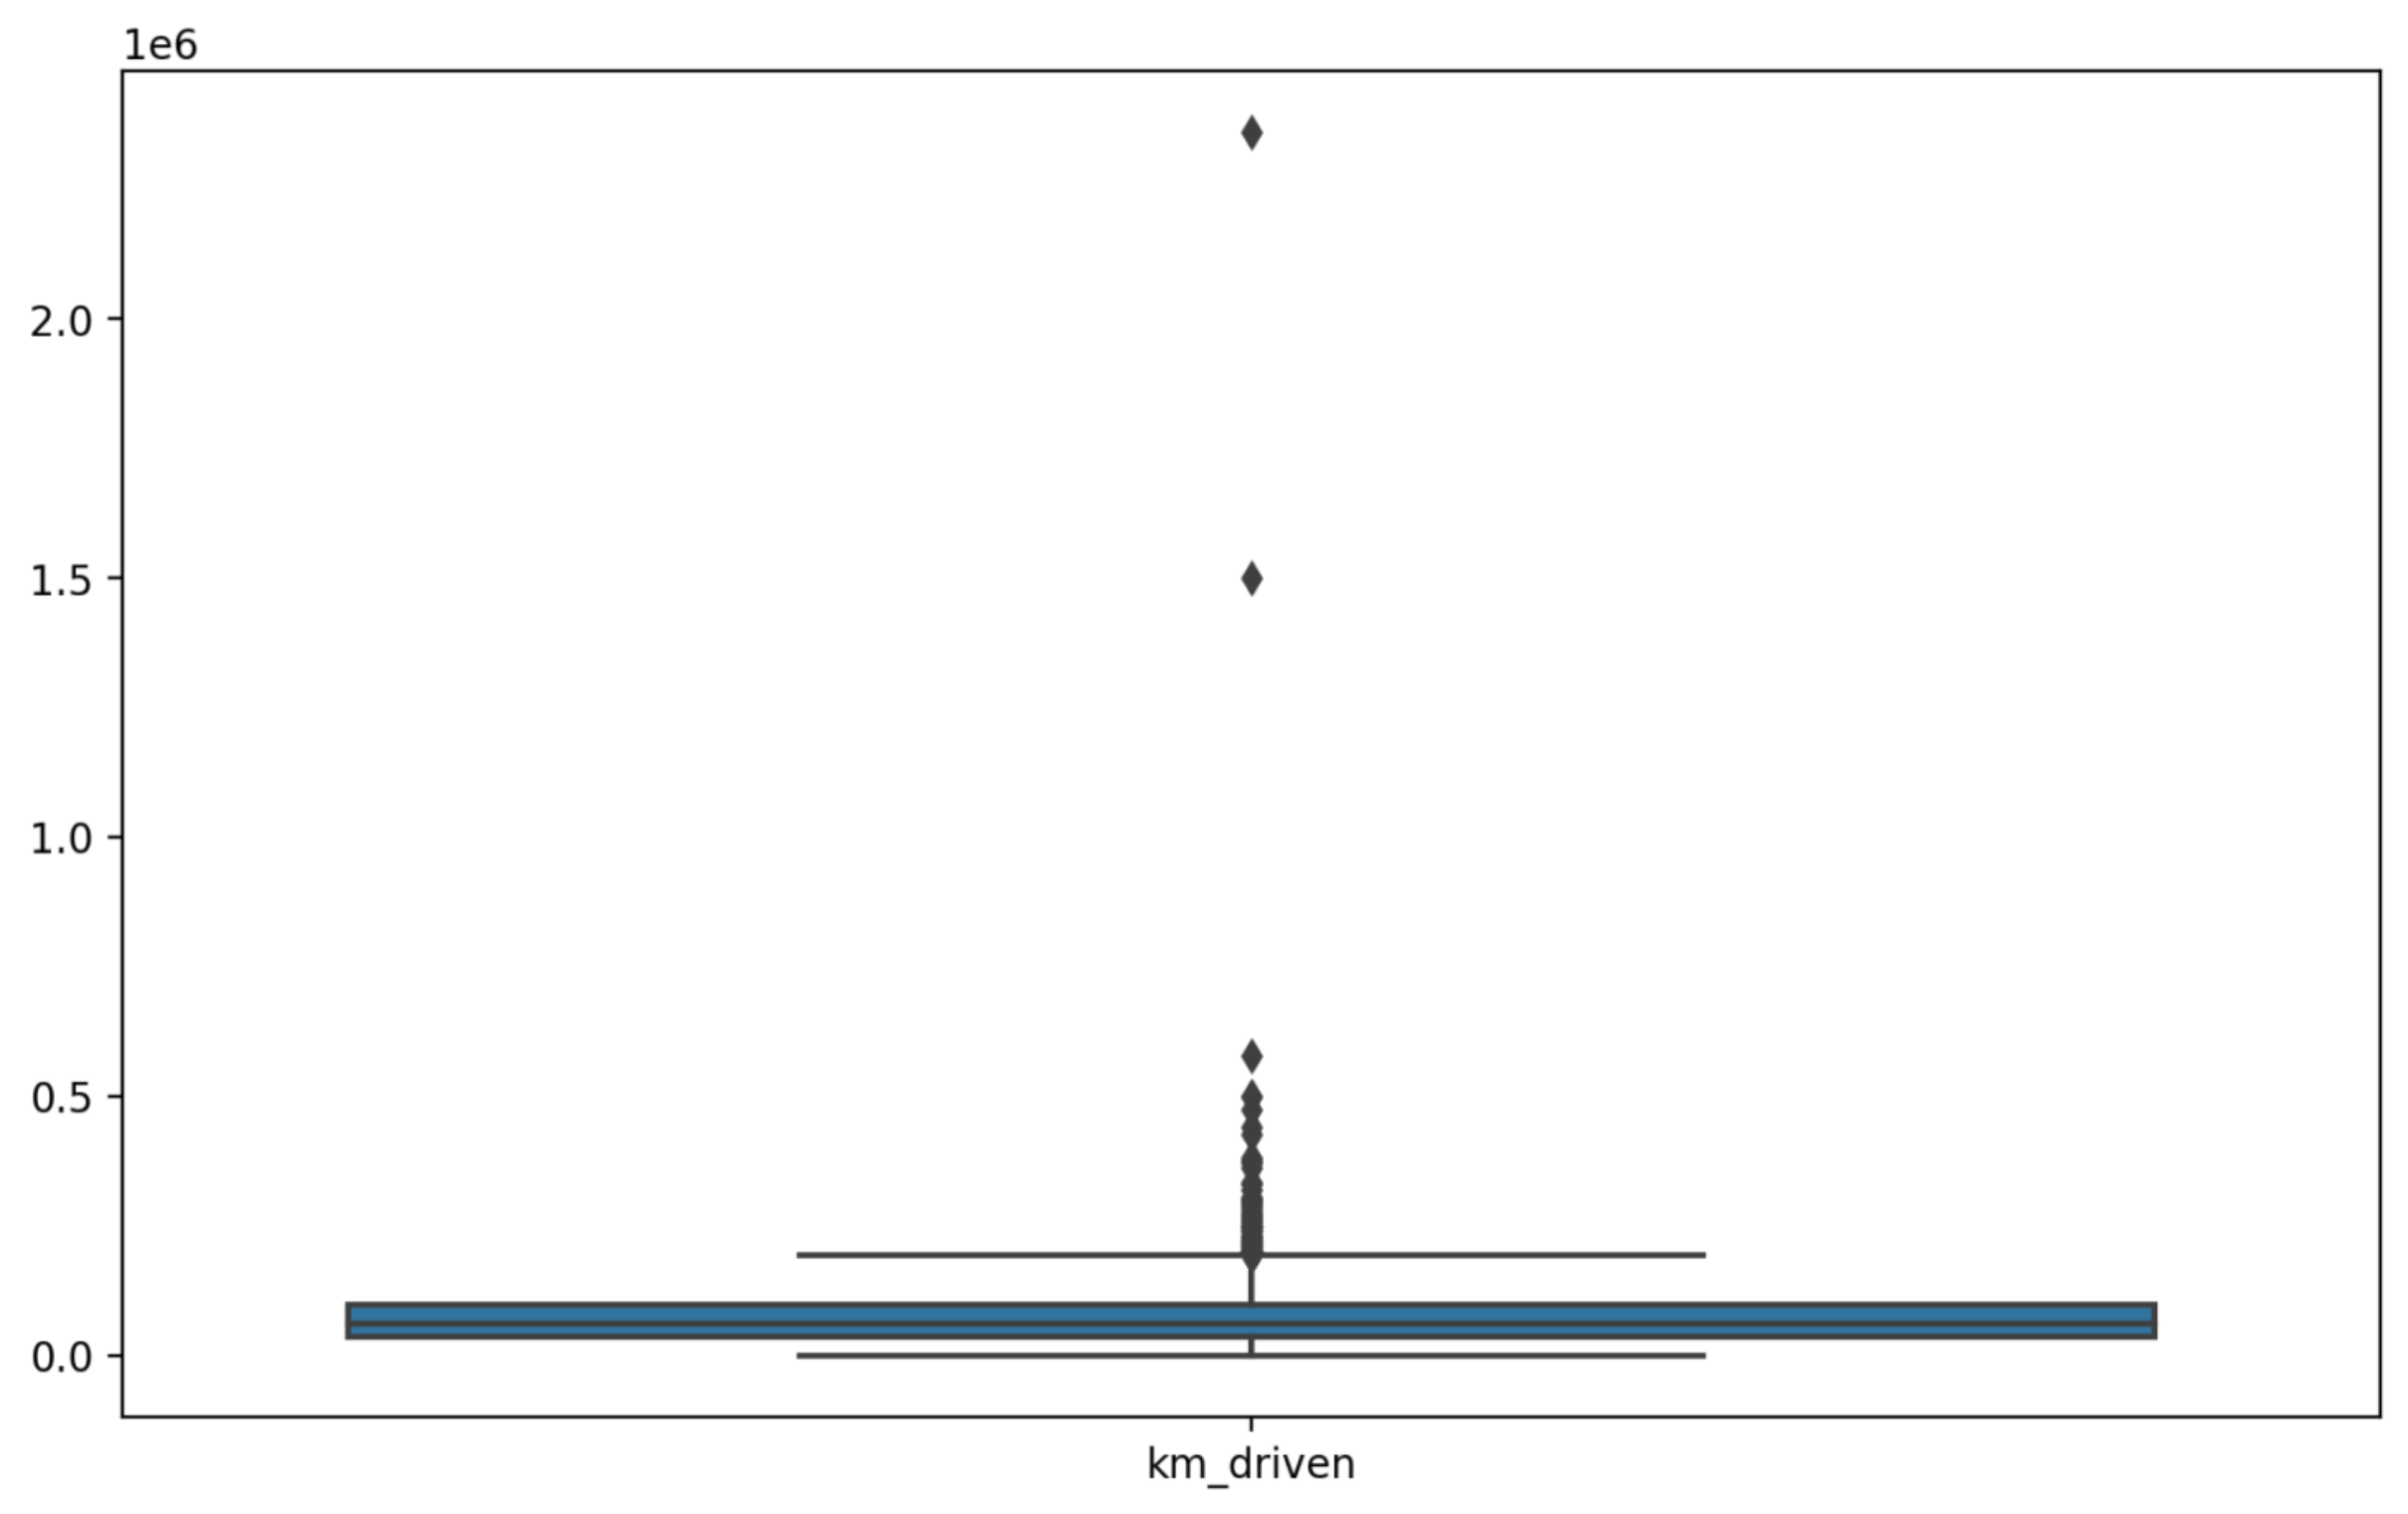
\includegraphics[width = .4\textwidth]{Figuras/Before Boxplot.png} 
\caption{Box plot before outlier removal}
\end{figure}
    
\begin{figure}[h]
\centering
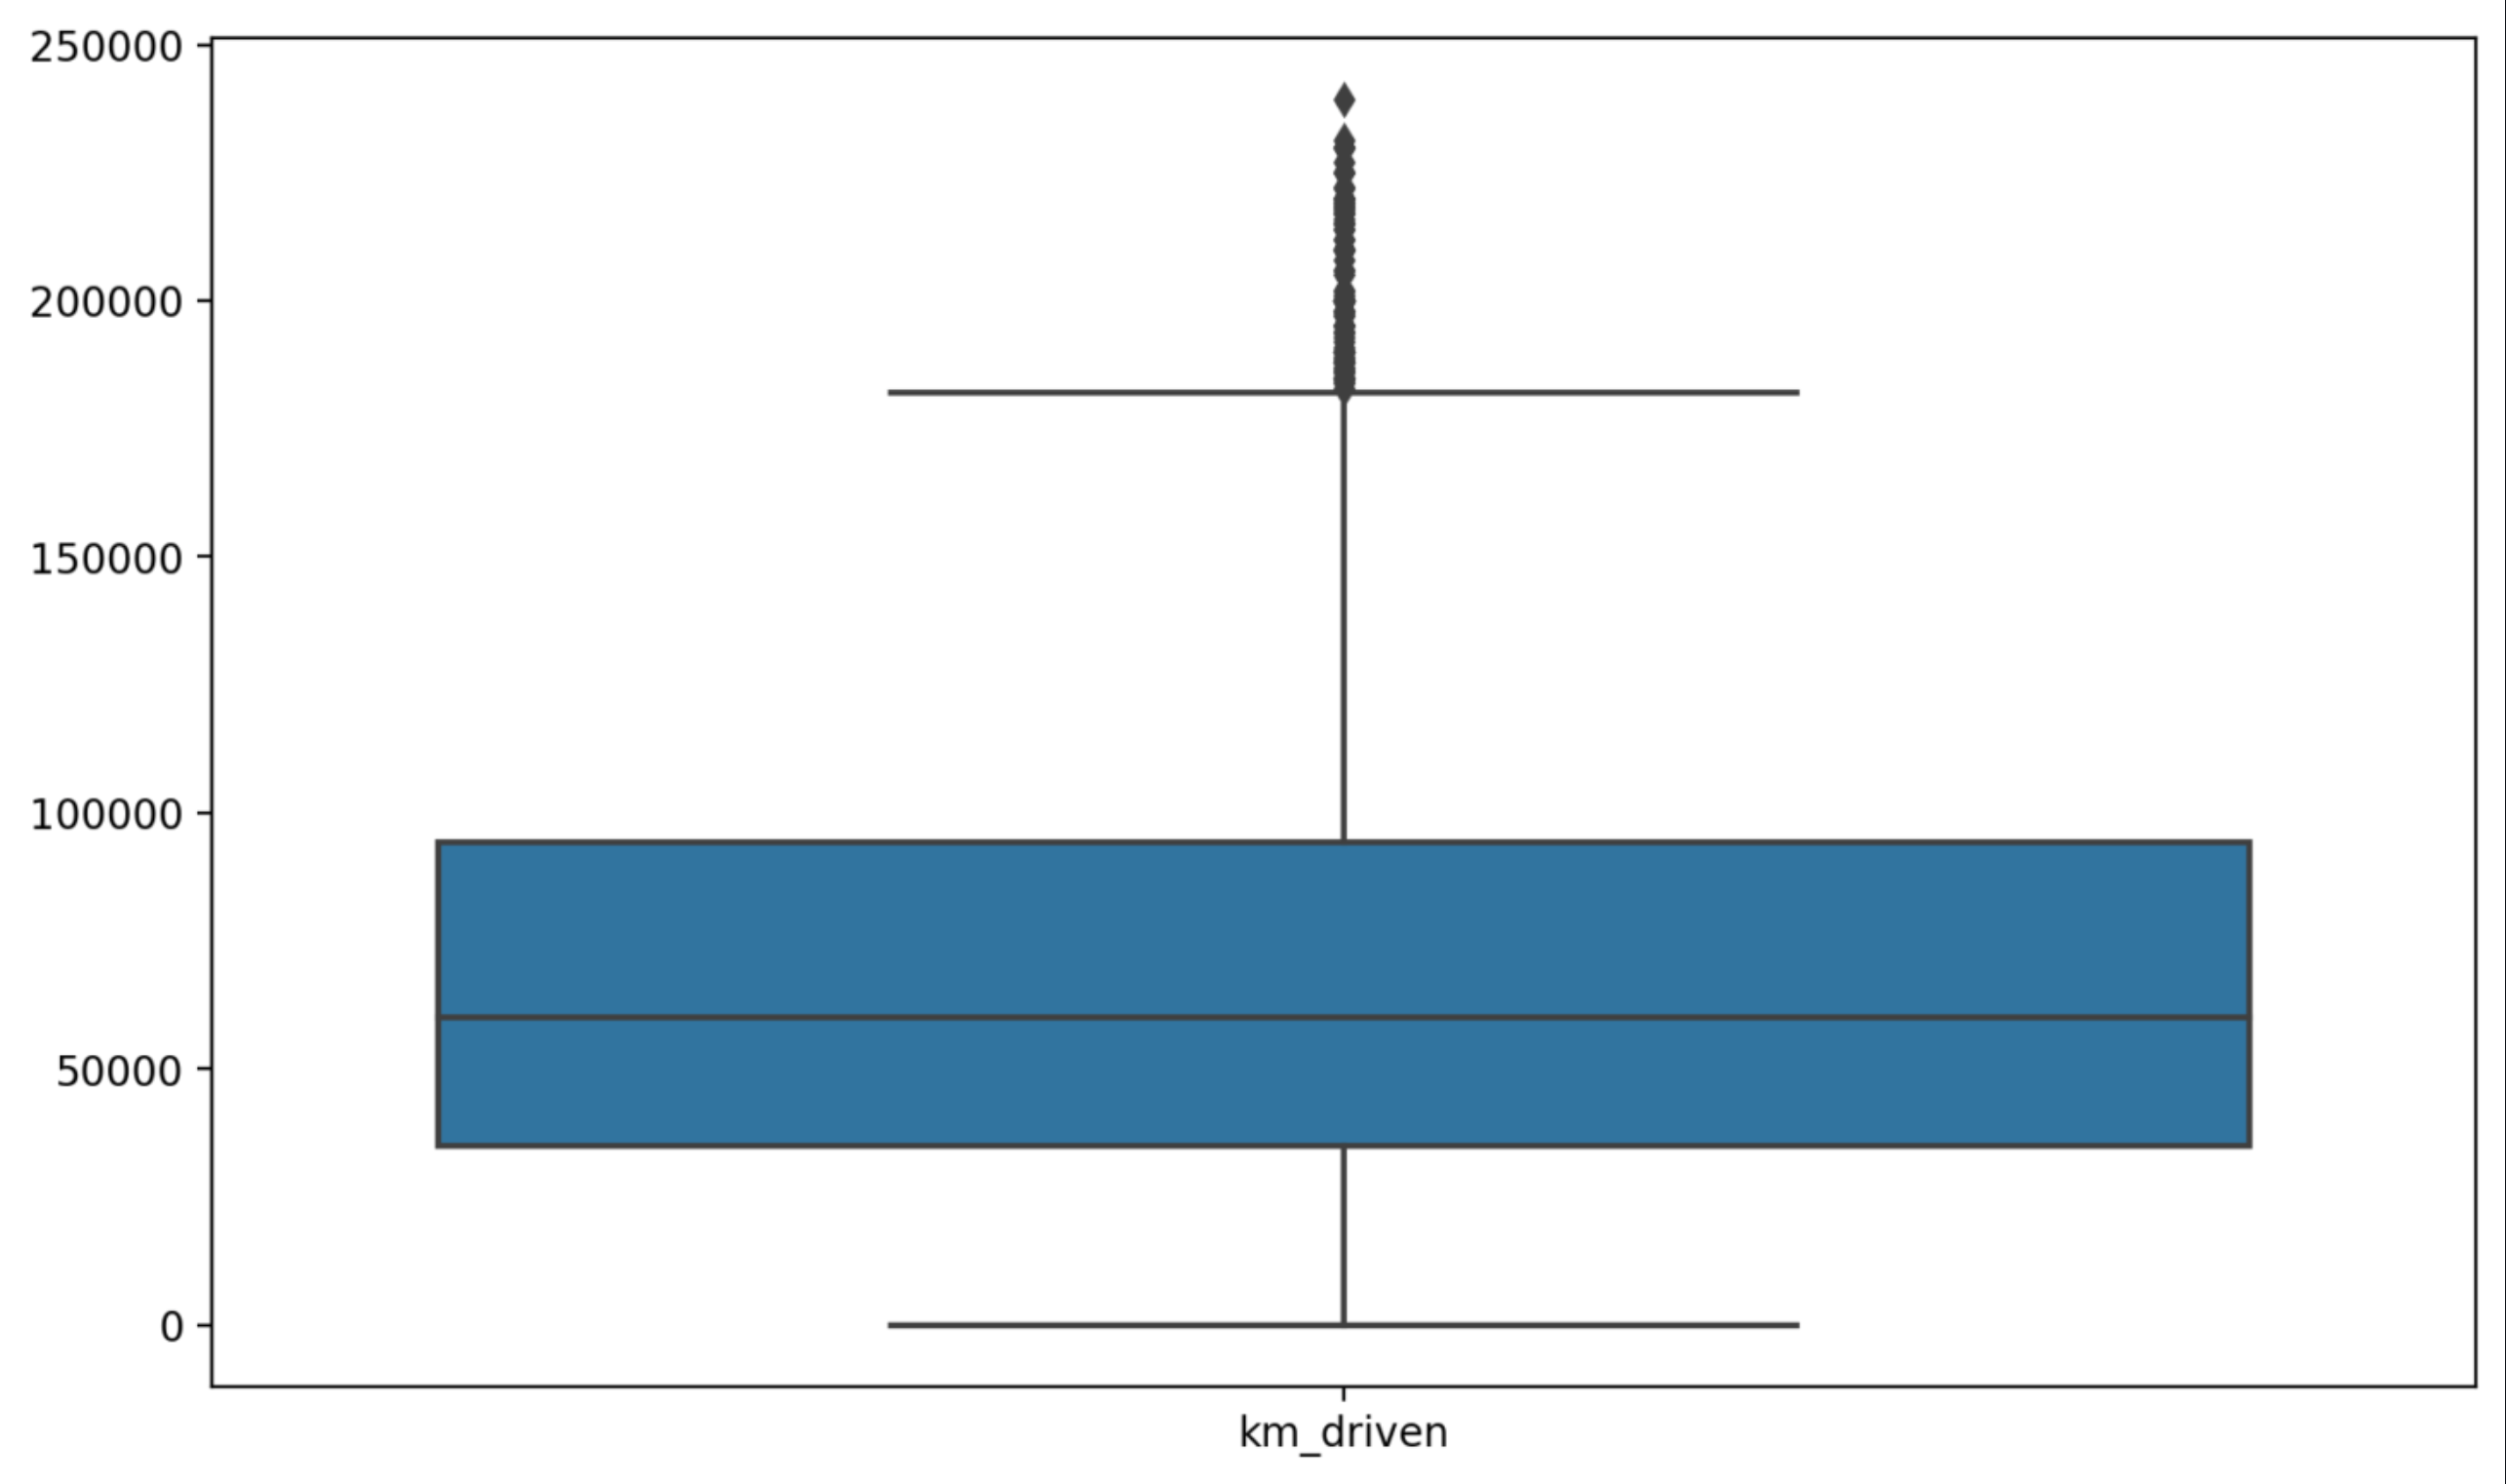
\includegraphics[width = .4\textwidth]{Figuras/After Boxplot.png}
\caption{Box plot after outlier removal}
\end{figure}

Further, the tab allows users to normalize or standardize data. The min-max method performs the data normalization, which maps the data into a range of 0 to 1. This makes model training less sensitive to the scale of the features, which allows the model to converge to better weights and leads to a more accurate model\cite{normalization} \[X_{\text{norm}} = \frac{X - X_{\text{min}}}{X_{\text{max}} - X_{\text{min}}}\]. Before implementation of a distance-based classifier like K nearest neighbors, the standardization is required to make all variables contribute equally to similarity measure \cite{standardization} \[Z = \frac{X-\mu}{\sigma}\]. 

\subsection{Second Tab}


The second tab of the projects is dedicated to data visualization. After processing data, users can generate different visualizations. Users are prompted to select the type of visualization, such as a histogram, bar chart, line chart, scatter plot, or heatmap. Following the selection of visualization, users can specify the corresponding columns if needed and make personal modifications like color changes or adding hue to the scatter plot. The title of the visualization is added automatically after the choice of columns. The visualizations are generated using Matplotlib and Seaborn Python libraries. 




\subsection{Third Tab}

Users can create personalized fraud detection tools after processing data and getting helpful information from the data. As banks and companies have different standards, it is essential to have a tool that will operate on those standards. After uploading the dataset, it automatically gets encoded for future processing. Users are asked to select features on which the machine learning algorithms will train and the target variable that will be predicted. Further, users are requested to choose the ML algorithm on which they want the data to be operated. Three algorithms are provided for selecting: Random Forest, XGboost, and SVM. After training the algorithm on the data, users can see the model evaluation, which contains information about the accuracy score, classification report, and confusion matrix. After this step, users can upload new transaction datasets that are not labeled for prediction. A new column named predictions will be added to new datasets, which will label the new transactions as fraudulent or legitimate as 1 and 0 accordingly. 



\subsubsection{Random Forest}

Random Forest is a supervised machine learning algorithm used for classification. It constructs a group of decision trees of the training data and matches them with test data. The advantage of the random forest is that it uses many decision trees to improve the predictions instead of one decision tree. As a result, the random forest employs a bagging method to generate a forest of decision trees. Given a dataset (X,Y) with N total observation where X being the predictor variables, and Y the outcome variable, the random forest algorithm first creates \(K_i\) random variables \((i = 1,2,...,N)\) to form a vector and then, it converts each \(K_i\) random vector into a decision tree to obtain the \(dK_i\) decision tree \(dK_1(X),dK_2(X),...,dK_N(X)\) The final classification results are as follows:\cite{afriyie2023supervised} \[D(X) = argmax( \sum_{i=1}^N dK_i(X) (K_i = \text{Fraud}) +\]  
\[\sum_{i=1}^N d_i(X) (K_i = \text{Not Fraud}))
\]

The model correctly predicted 19946 legit transactions as not fraudulent, two transactions were incorrectly predicted as fraud, 40 fraudulent transactions were correctly detected, and 12 transactions were mispredicted as legit. 

\begin{table}[h!]
\centering
\begin{tabular}{||c c c c c||} 
 \hline
 Accuracy & Precision & Recall & F1-score & Support \\ [0.5ex] 
 \hline\hline
 \textbf{99.93} & \textbf{0.95} & \textbf{0.77} & \textbf{0.85} & \textbf{52} \\ 
 \hline
\end{tabular}
\caption{Classification report of the random forest model}
\label{table:1}
\end{table}





\subsubsection{XGboost}

Extreme Gradient Boosting or XGBoost is another classification method that can perform various functions such as regression classification and ranking. The most crucial advantage of XGBoost is its scalability.\cite{permai2023prediction} The algorithm works by sequentially adding weak learners to the ensemble, with each new learner focusing on correcting the errors made by the existing ones. It uses a gradient descent optimization technique to minimize a predefined loss function during training.\cite{XGboost} The XGBoost algorithm is known for its high accuracy compared to other algorithms. Nevertheless, the algorithm works faster by using multiple cores to build decision trees faster. It gathers information about all data points at once and then splits them up for processing across multiple cores. 


The model correctly predicted 19947 transactions as legit, 1 transaction was incorrectly predicted as fraudulent, 43 fraudulent transactions were detected, and 9 fraudulent transactions were not detected.


\begin{table}[h!]
\centering
\begin{tabular}{||c c c c c||} 
 \hline
 Accuracy & Precision & Recall & F1-score & Support \\ [0.5ex] 
 \hline\hline
 99.95 & 0.98 & 0.83 & 0.9 & 52 \\ 
 \hline
\end{tabular}
\caption{Classification report of the XGboost model}
\label{table:2}
\end{table}



\subsubsection{SVM}

A support vector machine or SVM is another supervised machine learning model for classification or regression problems. They handle linear and nonlinear data by finding the hyperplane that best divides the data into classes. The key idea behind SVMs is to transform the input data into a higher-dimensional feature space. To do this, SVMs use a kernel function. Instead of explicitly calculating the coordinates of the transformed space, the kernel function enables the SVM to implicitly compute the dot products between the transformed feature vectors and avoid handling expensive, unnecessary computations for extreme cases.\cite{SVM} The support vector machine classifies new data points better when there are clear separations between classes and is memory efficient. However, it only works well with large datasets. 

The model correctly predicted 19943 legit transactions, 5 legit transactions were predicted as fraudulent, 19 fraudulent transactions were detected, and 33 fraudulent transactions were incorrectly predicted as legit. 


\begin{table}[h!]
\centering
\begin{tabular}{||c c c c c||} 
 \hline
 Accuracy & Precision & Recall & F1-score & Support \\ [0.5ex]
 \hline\hline
 \textbf{99.81} & \textbf{0.79} & \textbf{0.37} & \textbf{0.5} &\textbf{52} \\ 
 \hline
\end{tabular}
\caption{Classification report of the SVM model}
\label{table:3}
\end{table}



\section{Conclusion And Future Work}

With the growth of online transactions worldwide, risk management, especially fraud detection, has become more complicated than ever. Non-technical solutions often show wrong results. Hence, modernization of this field is urgent -the project aimed to study and develop a user-friendly tool for non-technical risk managers and compliance officers. 
In conclusion, tree models were implemented and tested on the abovementioned dataset. According to the results, the best performance showed the XGboost algorithm, and the worst result showed the SVM algorithm. In the future, time series analysis tabs can be developed to let users implement complex time series analysis models on specific datasets. Moreover, unsupervised and hybrid models can be explored and tested as well.


\clearpage
\bibliographystyle{unsrt}
\bibliography{mybib}

\end{document} 